\section{On-demand open-world evaluation}
\label{sec:methodology}

We have shown that the bias in a closed-world evaluation poses an obstacle to innovating new systems.
We could eliminate the bias if we had exhaustively annotated the entire document corpus so that any relations predicted by systems would already be annotated.
Unfortunately, this would be a laborious and expensive task: for a collection of 10,000 documents, we estimate that it would cost at least \$300,000 if non-expert annotators were employed.

In on-demand open-world evaluation, the evaluation process is automated so that new relations can be annotated on-demand.
Once a new system or feature has been developed, its predictions can be submitted to an evaluation portal.
Behind the scenes, the predicted relations are sampled to be evaluated.
If the relation is outside the current evaluation set, annotations are immediately obtained through crowd-sourcing and added into the evaluation set.
Thus, we push the hard work of finding candidate relations to automated systems and instead focus annotation effort on the much easier task of verifying relation predictions.
At the end of this process, systems obtain fair instance-level, relation-level and entity-level scores.

%On the other hand, it is much easier to verify a relation instance predicted by a system.
% TODO: outline the structure of the framework better.
% TODO: this should mention pooled annotations, etc.
There are two further problems we must address. %three inter-related challenges that we must tackle.
First, we must ensure that our estimates of recall accurately reflects open world scores despite being evaluating on an evaluation set constructed from system predictions.
%  We achieve this by calibrating our scores on a small set of exhaustively annotated documents.
Secondly, we must ensure that the relations we sample allow us to compute unbiased entity-level and relation-level precision scores.
%  We achieve this through structured sampling.
%$Finally, we would to implement our evaluation framework cost-effectively.
%  We achieve this by combining annotations across systems and sampling schemes through importance reweighing.
We discuss our solutions to these problems next.

\subsection{Ensuring open-world recall with exhaustive annotations}
% A line about pooled recall
The pooled collection of evaluated relations in the evaluation set is unlikely to be an accurate estimate for all the true relations in the corpus and thus the pooled recall would be a biased estimate.
At the same time, it is impossible to know how many true relations there are in the corpus without annotating it in its entirety.
We address this problem by obtaining exhaustive annotations on a few documents to correct for the bias in using pooled recall.
% vv is possibly too much detail.
%For each sampled document, a crowdworker annotates any entities he/she can find.
%In a separate task, crowdworkers are then asked to identify relations between every pair of mentions in a single sentence.
%%\footnote{%
%%While there certainly are relations across sentences, this requires crowdworkers to evaluate many more mention pairs for relations.}
%During entity annotation, crowdworkers also link entities to Wikipedia pages if possible, allowing us to perform entity-level evaluation.

%We first evaluate whether exhaustive annotations can be reliably performed by crowdworkers.
%To do so, we compare crowdsourced annotations against those of expert annotators using data from the TAC-KBP 2015 EDL task~\citep{}.\footnote{%
%Further details regarding the annotation interface and experiment can be found in \refsec{turk}.
%}
%We find that crowdworkers identify 90\% of the entity spans identified by expert annotators and have significant token-level inter-annotator agreement (\fake{$\kappa = 0.8$}), validating the hypothesis that exhaustive annotation crowdsourced.

Then, when evaluating recall, we first estimate recall of the entire evaluation set on the exhaustively annotated documents, and multiply that by the recall of the system on the evaluation set. Through this two-step process we exploit the fact that it is easier to reduce variance by increasing the size of the evaluation set than it is to increase the size of the exhaustive annotation. \refsec{power} provides more details about this variance reduction.

A final issue to discuss is how documents should be sampled to capture diverse entities that span documents. % to provide better entity-level scores.
When considering uniformly sampled documents, we that find that only extremely frequent entities like the United States or Barack Obama appear across documents.
Unfortunately, we do not know which entities are present in which documents to construct a fairer sampling scheme.
As a heuristic, the 20\% of our exhaustive document collection is sampled uniformly and annotated.
We then uniformly sample the entities annotated to create a collection of ``query entities''.
Finally, we construct the remaining 80\% of our document collection by searching for documents that contain the query entities according to an exact string match.
% TODO: would be nice to quantify 

\subsection{Structured sampling for entity-level and relation-level precision}
Estimation of relation-level and entity-level scores respectively assumes that relation types and entities are sampled uniformly.
However, if we were to uniformly sample relations from a typical system's predictions, 
  we would get a very skewed distribution over relation types and entities and thus bias our estimates.
We address this problem through two structured sampling schemes.

First, for relation-level scores, we stratify the predicted instances by relation and collect the same number of samples from each relation.
Secondly, for entity-level scores,  we first sample subject entities uniformly from the predicted KB, then sample fills for that entity, followed by instances for the fill.
For each such entity, we draw several samples.
% TODO: show a diagram.

Similarly, the distribution over relation instances for each system and scoring scheme (i.e.\ entity-level and relation-level) will be quite different. We correct for bias through importance reweighing~\citep{}.

%In \sectionref{analysis} we identified two main problems with the current evaluation methodology:
%\begin{enumerate}
%  \item A closed-window pooling evaluation is significantly biased
%    against development systems, particularly those of new teams.
%  \item Existing evaluation metrics have too much variance on the
%    evaluation data to be a measure of performance that will generalize
%    to new documents and queries.
%\end{enumerate}
%
%At the same time, we would like to capture some of the defining aspects of the original TAC-KBP evaluation:
%\begin{enumerate}
%  \item The evaluation should allow comparisons against human effort on the task. %TODO: reason?
%  \item Scores should be aggregated over entities, because entity-level scores are a more natural measure of knowledge base quality.
%  \item Teams should be required to submit justifications for relations they predict, because this makes it possible to interpret and verify system output.
%\end{enumerate}
%
%Our goal in this section is to propose a new methodology that maintains the above elements while addressing the mentioned problems head on 
%  by indefinitely opening the pooling evaluation window by making the evaluation online \pl{not sure what this means}
%  and by combining evaluation data for each team in statistically optimal fashion.
%Before we describe the overview of our proposed evaluation platform, we take a brief detour to answer an important question.
%
%\paragraph{Would a larger human-annotated dataset suffice?}
%A natural question to ask before embarking on the significant effort of an online evaluation is whether a large-enough dataset could be reliably collected by spending a little more money. 
%
%An important part of the KBP evaluation is to test on an unseen document collection.
%
%A number of datasets for relation extraction, even on the TAC-KBP task, have been collected in the past, for example in the work of \citet{angeli2014combining}.
%This dataset is very small \pl{quantify} and does not have sufficient coverage, but is useful for training \pl{strange - usually test set is smaller than training}.
%Unfortunately, these datasets have also been collected by pooling responses. \pl{clarify what this means}
%
%Another way of empirically answering this question is to see how many contexts need be evaluated to reduce pooling bias sufficiently. We can extrapolate this number by studying how the pooling bias varies by the number of systems.
%Using the 2015 evaluation data, we find that we would need to pool the output of \fake{100} systems with \fake{$10^6$} lines of output \pl{what is line of output?} evaluated.
%\pl{not clear what is being computed or how to think about this}
%With the `anydoc' heuristic, this number is far less, but the error introduced by the heuristic also increases.
%%TODO: graph.
%
%We can estimate the cost of annotating such a large corpus by calculating how many documents need be exhaustively annotated by humans-- it comes out to \fake{\$100,000}. 
%We believe this is reasonable justification to discard the static dataset approach and embrace an online evaluation wherein systems are continuously evaluated.

% \paragraph{Overview of the evaluation platform.}
% The interface to our proposed evaluation platform is very similar to that of the TAC-KBP competition:
% % input?
%   participating teams are provided a document corpus with about $10,000$ documents
% % output?
%   and asked to submit a knowledge base consisting of every entity mention in the document along with links to canonical entity ids and relations between these entity mentions.
% However, unlike the TAC-KBP competition, the submitted knowledge base is immediately evaluated for correctness and coverage by crowdworkers.
% % metrics?
% Teams obtain mention-level and entity-level scores within hours of their submission, allowing them to improve their systems immediately.
% After several months of submissions, we plan to release the data annotated during this evaluation period and move on to a new evaluation corpus. 
% 
% There are two other significant departures from the current KBP specification.
% First, we ask teams to submit every relation context justifying a predicted relation between two entities instead of just one:
%   this additional output will be valuable in measuring the relation extraction quality independent of entity linking performance.
% % queries?
% Secondly, we evaluate entity-level scores on randomly sampled entities from documents instead of manually constructed queries.
% The queries developed by the LDC were explicitly designed to be challenging, but unfortunately this is a subjective criterion that is hard to automate-- \fake{we show later that queries that are randomly sampled are still quite challenging to state of the art systems.}
% Recent editions of the competition have included `two-hop' scores that evaluate how well the constructed knowledge base can answer queries that traverse two relational edges, e.g.\ ``What was Carrie Fisher's mother professional title?''
% Evaluation using these two hop queries is currently out of scope for this work.
% 
% Next, we will describe how crowdworkers evaluate the submitted output, starting first with precision and followed by recall.
% 
% \begin{figure*}
% \begin{subfigure}{0.31\textwidth}
%   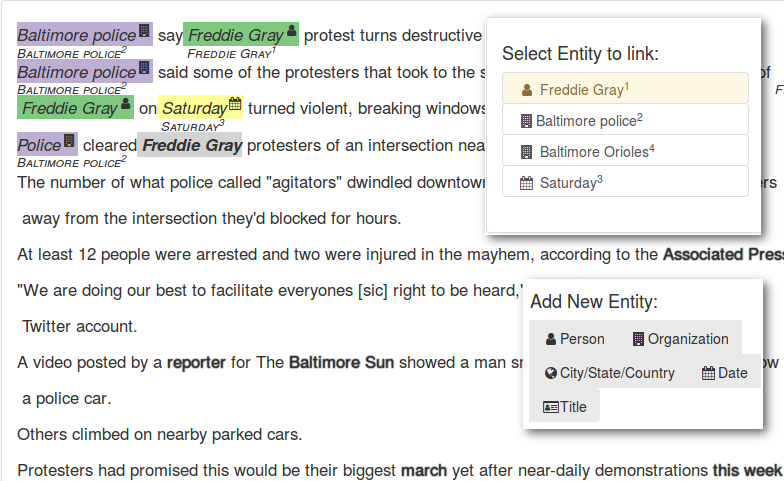
\includegraphics[width=\textwidth]{figures/extraction-interface}
%   \caption{\label{fig:entity-interface} Entity detection and linking.}
% \end{subfigure}
% \hfill
% \begin{subfigure}{0.31\textwidth}
%   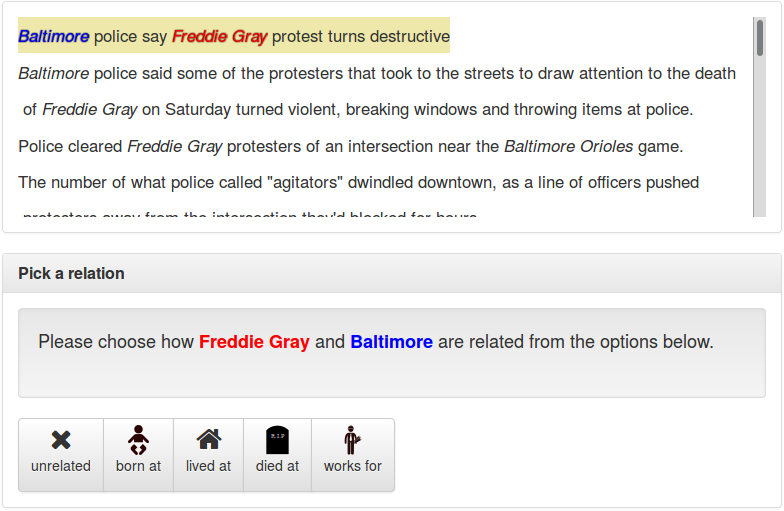
\includegraphics[width=\textwidth]{figures/relation-interface}
%   \caption{\label{fig:relation-interface} Relation extraction.}
% \end{subfigure}
% \hfill
% \begin{subfigure}{0.31\textwidth}
%   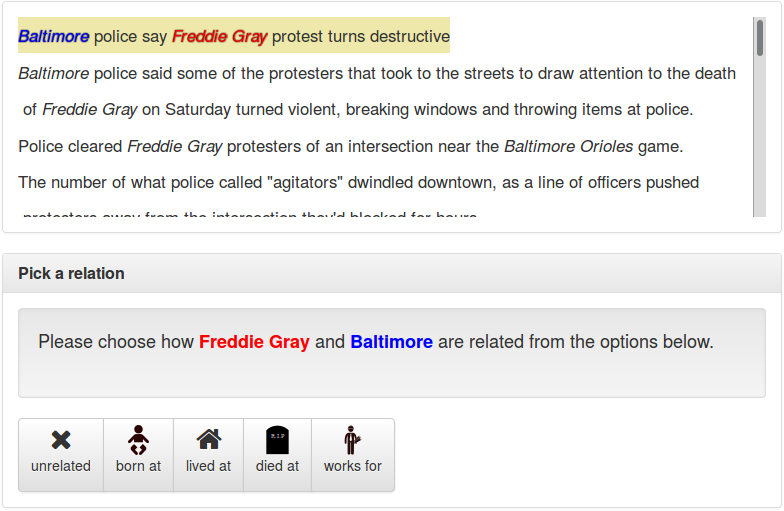
\includegraphics[width=\textwidth]{figures/relation-interface}
%   \caption{\label{fig:linking-interface} Cross-document linking.}
% \end{subfigure}
% \caption{\label{fig:interfaces} Screenshots of the annotation interfaces.}
% \end{figure*}
% 
% % TODO: Report entropy of our entity selection?
% 
% % Basically, why do it document based versus query based?
% % TODO: Report recall of our entity annotation
% % TODO: Report "entropy" of our entity annotations -- are they more "diverse" than LDC's?
% 
% \paragraph{Evaluating precision with pooled annotation.}
% % Actual interface to verify turker output.
% Entries in the submitted knowledge base are verified by crowdworkers using the context provided.   
% Using an annotation interface shown in \figureref{relation-interface},
% crowdworkers are asked to verify 
%   whether the participating mentions in the relation are valid entities,
%   whether the predicted relation holds between the two mentions and
%   whether the mentions are correctly linked if the mention is linked to a Wikipedia entry.
% If the participating mention is not linked to a Wikipedia entry,
% then we ask crowdworkers to resolve cluster assignments using a separate interface (\figureref{linking-interface}).
% On average, we find that crowdworkers are able to perform this task at about 10 seconds an entry, corresponding to about \$0.03 per entry, and we need about \fake{3 workers per entry} to achieve an inter annotator agreement of \fake{0.90}.
% 
% % We need to sample output.
% Each system may output many thousands of relations-- evaluating every one of these relations would be prohibitively expensive
%   and ultimately unnecessary if we are willing to only provide metric scores up to a certain degree of confidence.
% % How much output to sample?
% We propose instead to sample predicted relations and their contexts from each system's output to achieve a desired confidence interval.
% % how to extend to entities?
% However, uniformly sampling over entries would cause popular entities to be overrepresented in our entity-level scores.
% Instead, we first uniformly sample entities from the output, then sample fills from each entity and mentions for each fill (see \figureref{evaluation-table} for a visual representation of this clustering).
% Precision scores of each fill (measured over its mentions) are aggregated to compute the precision score of that entity.
% It is easy to reuse these stratified samples to evaluate mention-level metric scores using importance reweighing. 
% Annotating 1,000 contexts is sufficient for a confidence interval of about 3\% points and comes at a much more reasonable cost of about \$100 for a submission. 
% % how to reuse labels and amortize costs?
% Furthermore, we can reuse annotations on entries from previous submissions\footnote{
% These annotations must be importance reweighed to eliminate bias.},
%   allowing the cost per submission to decrease with increasing numbers of submissions.
% 
% \paragraph{Evaluating recall with exhaustive annotation.}
% The pooled collection of relations from submissions is unfortunately still a very poor proxy for the set of all possible relations in the document corpus.
% Consequently, we propose having crowdworkers attempt to exhaustively annotate entities and relations on a random sample of about 100 documents.
% Crowdworkers begin by identifying every mention span in a document and specifying its type using the interface shown in \figureref{entity-interface}. For each mention, they are also asked to identify the canonical mention (i.e.\ perform coreference) within the document and identify links to Wikipedia pages.
% Every pair of mentions within a sentence\footnote{
%   We found that an overwhelming majority of relations were expressed in a single sentence.
%   The quadratic blowup in overhead of considering mentions across two sentences is simply not worth it.}
%   with compatible types is then shown to a crowdworker, who is then requested identify the relation between the two mentions using the relation identification interface (\figureref{relation-interface}).
%   Finally, we ask crowdworkers to cluster entities that could not be linked to Wikipedia using the clustering interface (\figureref{linking-interface}).
%   In this interface, crowdworkers are shown canonical mentions for every unlinked entity cluster from the small document corpus.
% 
% These interface are far more involved and consequently take longer for crowdworkers to complete.
% The entity annotation interface takes on average about 10 minutes per document, corresponding to about \$2.00 a document, and 
% again required \fake{3 annotators} to get to an inter-annotator agreement of \fake{0.90}.
% The relation annotation interface takes on average about 3 minutes per document, corresponding to about \$0.60 a document, and required \fake{3 annotators} to get to an inter-annotator agreement of \fake{0.90}.
% Finally, the clustering interface takes on average about \fake{6 minutes for 100 documents}, corresponding to about \fake{\$1.20 a document}, and required \fake{3 annotators} to get to an inter-annotator agreement of \fake{0.90}.
% On average, there are about \fake{10 relations a document} and it costs about \fake{\$0.36 a relation} through the exhaustive interface.
% 
% There are two simplifications we adopt in our interfaces.
% Firstly, we exclude the extremely rare relations corresponding to ``cause of death'', ``has criminal charge'', ``age'' and ``number of employees'' and correspondingly their slot types.
% In total, annotators specify one of five types, ``Person'', ``Organization'', ``City, State or Country'', ``Date'' and ``Title'', with the latter being a very common example of an open-category non-named type.
% Secondly, we do not allow crowdworkers to annotate nested spans, preventing them from identifying both the organization and the city in \textit{``[University of [Chicago]]''}. 
% 
% Unfortunately, a uniformly random sample of documents from the corpus is unlikely to contain any cross-document links for any but the most popular of entities.
% Consequently, while constructing the document collection, we first randomly sample about 20 documents and annotate them.
% From the set of named entities identified, we uniformly sample (without replacement) an entity and then uniformly sample up to 4 additional documents that mention this entity by name and annotate them.
% We repeat this procedure until we have 100 documents.
% While this sampling procedure is not representative of the whole corpus, it does increase the probability of having cross-document links for less popular entities, capturing that criteria from the TAC-KBP evaluation queries.
% 
% \paragraph{Reducing variance by incorporating pooled and unassessed output.}
% We have just seen that identifying a relation through exhaustive annotation scheme costs about 10 times as much as it does to verify a predicted relation.
% Given this price differential, it is tempting to consider using the recall of a system measured against the pooled output instead of measuring the true recall.
% However, if use the exhaustive annotation to compute the \textit{recall of the entire pool}, we can in fact use \textit{pooled annotations} and the \textit{unassessed output} to better estimate \textit{true recall}.
% 
% \begin{figure*}
%   \begin{subfigure}{0.49\textwidth}
%     \caption{\label{fig:variance-reduction}}
%   \end{subfigure}
%   \begin{subfigure}{0.49\textwidth}
%     \begin{tabular}{l r r r r} \toprule
%       Scheme     & Cost   & $E\oft{p}$ & $E\oft{e}$ & Total cost \\ \midrule
%       Exhaustive & \$0.36 &   & 1 & \$1000 \\
%       Pooled     & \$0.03 & 1 &\fake{3} & \$1000 \\
%       Unassessed & \$0.00 & \fake{0.5} & \fake{0.5} & \$0 \\
%       Hybrid     & \fake{\$0.10} & \fake{1.5} & \fake{4.5} & \$1000 \\ \bottomrule
%     \end{tabular}
%     \caption{\label{tbl:variance-reduction}}
%   \end{subfigure}
%   \caption{(a) A schematic to show how pooled and unassessed annotations can decrease the variance of predicting recall when combined with exhaustive annotations (see text). Green and red identify correct and incorrect contexts. 
%   (b) A summary of cost-accuracy tradeoffs of different annotation schemes described in the text.
%   The hybrid annotation scheme uses an optimal combination of the exhaustive, pooled and unassessed schemes.
%   The middle two columns describe estimated relative efficiencies of using the specified scheme versus only the pooled annotation scheme for precision ($E\oft{p}$) and versus only the exhaustive annotation scheme for recall ($E\oft{e}$).
%   The last column estimates the cost of using the specified scheme to annotate \fake{the entire document corpus}.
%   }
% \end{figure*}
% 
% Consider the following example for intuition (see \figureref{variance-reduction}).
% Let $E$ be the set of contexts that are exhaustively annotated,
%   $P$ the pooled set of contexts that have been annotated and 
% %  $U$ the pooled set of unassessed contexts and 
%   $S$ is the set of contexts submitted by a system.
% As earlier, let $C^*$ be the set of correct contexts (shown in green) and $\bar{C}^*$ be the set of incorrect contexts (shown in red).
% The recall of a system $A$ is the proportion of correct contexts it predicts, i.e. $R_A = \frac{|S \intersection C^*|}{|C^*|}$.
% However, because $S \subseteq P$, we can also describe its recall to be the product of the recall of $A$ within the pool and recall of the pool itself: 
%   $R_A = \frac{|S \intersection P^*|}{|P^*|} \frac{|P^*|}{|C^*|}$, where $P^* \eqdef P \intersection C^*$ is the set of correct entries within the pool, identified by pooled annotation.
% 
% Both these methods of computing recall have the same value in expectation, but may differ in variance; let's compare these now.
% Let $\hat{R}_A\oft{e}$ be an estimator of $R_A$ using only exhaustive annotations, 
%   $\hat{R}_P\oft{e}$ be an estimator of the recall of the pool, $R_P$, using only exhaustive annotations, 
%   $\hat{S}_A\oft{p}$ be an estimator of the pooled recall of $A$, $S_A$, using pooled annotations and 
%   $\hat{R}_A\oft{p} = \hat{R}_P\oft{e} \hat{S}_A\oft{p}$ be an estimator of $R_A$ that combines exhaustive and pooling annotations.
%   To first order, the variance of recall is determined only by the number of contexts annotated and thus the variance of $\hat{R}_A\oft{e}$ and $\hat{R}_P\oft{e}$ are about the same.
%   Also, given that it is very easy to annotate many more contexts with a pooled scheme, let us assume that the variance of $\hat{S}_A\oft{p}$ is practically zero.
%   Then, the variance of $\hat{R}_A\oft{p}$ is (again, to first order) basically $(\hat{S}_A\oft{p})^2$ times the variance of $\hat{R}_P\oft{e}$-- in other words $\hat{R}_A\oft{p}$ is less than $\hat{R}_A\oft{e}$ by a factor of $(\hat{S}_A\oft{p})^2$!
% Intuitively, if the recall of a system is very small compared to its pool we should hope to reliably estimate its recall using the pool.
% On the other hand, if it is large relative to the pool, the pooling annotation is unlikely to help.
% % TODO: address concern of valuating the recall of a perfect system poorly.
% In a similar way, we can also use agreements between the unassessed output of different systems to estimate recall within the unassessed pool, $U$.
% %For example, let us assume that, on average, half of the unassessed output is predicted by only one system and is true only 10\% of the time and that the other half of the unassessed output is predicted by at least 2 systems and is true 20\% of the time-- both these numbers can be estimated using the pooled annotations.
% %If our system only predicts half of the first part and two-thirds of the second, we can estimate that our system identifies $\frac{1}{10} \times \frac{1}{3}$ of the correct entries in the first part and $\frac{2}{10} \times \frac{2}{3}$ of correct entries in the second part. Furthermore, we can estimate that there are $\frac{1}{2} \times \frac{1}{10} \times U$ correct entries in the first part and $\frac{1}{2} \times \frac{2}{10} \times U$ correct entries in the second part.
% %Thus, our estimate of recall within this unassessed pool work out to be $\frac{1}{10}$.
% %Note that the variance of both of this recall prediction can be quite large, but can still nominally decrease variance of our predictions.
% 
% \tableref{variance-reduction} summarizes the variance reductions to be expected by combining pooled and unassessed annotations over using just exhaustive annotations, measured as relative efficiency.
% Note that the two estimators can always be combined so that the variance of the combination is less than the variance of each and that relative efficiency of the optimal combination of two or more estimators is simply the sum of their relative efficiencies.
% As a result, we can combine both pooled and unassessed annotations.
% The exact details are worked out in \sectionref{power}.
